\chapter{Implementation}
\label{cha:Implementation}

\section{Sprachen und Bibliotheken}

Die Python-Schnittstelle f"ur MCTDH wurde in der Programmiersprache Cython \cite{PyArt} erstellt. 
Cython stellt eine Hybridprogrammiersprache dar,
die Python und C\textbackslash C++ kombiniert. Im Gegensatz zu Python
wird Cython kompiliert, wobei die Cythonsyntax der Pythonsyntax "ahnlich ist.
In Cython kann C++ Code verwendet werden, der beim Erstellen der Cython-Programme ebenfalls kompiliert wird.
Auf diese Weise wurden mehrere Klassen in Python auf Basis von C++ Klassen erstellt.

Die GUI f"ur die MCTDH-Rechnungen wurde in Python mithilfe der Qt-Bibliothek implementiert.
Der Zugriff auf die Qt-Bibliothek \cite{Qt} erfolgt "uber die Python-Bibliothek PyQt4 \cite{PyQt}. 
Das Design der einzelnen GUI-Fenster erfolgte in Qt-Designer \cite{Qt-Designer}. Die Informationen "uber 
die jeweiligen Fenster werden in \textit{ui}-Dateien gespeichert. Mit PyQt k"onnen diese Dateien eingelesen werden und die entsprechenden 
Klassen erstellt und beliebig erweitert werden.
Die in Qt-Designer erstellten Fenster werden in PyQt miteinander verkn"upft.

Neben PyQt wurden die Python-Module \textit{networkx} \cite{SciPyProceedings_11} und \textit{matplotlib} \cite{Hunter:2007} verwendet.
Mithilfe von Klassen aus \textit{networkx} und \textit{matplotlib} konnten Baumdiagramme erstellt und gespei\-chert werden, die in der GUI zur 
Visualisierung des MCTDH-Baums verwendet wurden.

\section{Python-Interface f"ur MCTDH}
\label{sec:PyInterface}

Es wurde eine Programmierschnittstelle (von englisch \textit{application programming interface}, API) f"ur das MCTDH-Programmpaket erstellt,
welche es erlaubt den C++ MCTDH-Codes in Python-Skripten zu verwenden und in Python-Klassen zusammenzufassen.
Die Schnittstelle umfasst Klassen und Methoden, die zur Verwaltung der Darstellung der MCTDH-Wellenfunktion dienen.
Die Erweiterung auf andere Klassen kann nach einem einfachen Schema erfolgen.
Abbildung \ref{fig:uml_Cython} zeigt ein Klassendiagramm aller Klassen, welche "uber die API aufgerufen werden k"onnen.
Jede Klasse der API wird in Abbildung \ref{fig:uml_Cython} durch ein Rechteck repr"asentiert.
Im oberen Teil des Rechtecks ist der Klassenname angegeben und im unteren Teil sind die Methoden der Klasse aufgelistet.
Die baumartige Anordnung der Rechtecke repr"asentiert die Abh"angigkeit der Klassen zueinander. Eine Klasse h"angt von
allen Klassen ab, die sich im Diagramm unterhalb der betrachteten Klasse befinden und zu denen eine Verbindung besteht.
In der Klasse \textit{Controlparameters} werden die Genauigkeitsparameter der MCTDH-Rechnung verwaltet. 
Die Klasse \textit{physCoor} verwaltet Informationen einer Koordinate und enth"alt Informationen "uber das primitive Gitter oder
die primitive Basis. Sie ist ein Memberobjekt der Klasse \textit{mctdhNode}, welche einen Knoten im MCTDH-Baum 
repr"asentiert. In der Klasse \textit{mctdhNode} wird die lokale Konnektivit"at des Knoten, sowie dessen Satz von
Entwicklungskoeffizienten verwaltet. Die Dimensionen der Entwicklungskoeffizienten sind in Objekten der Klasse
\textit{Tdim} gespeichert. Die Klasse \textit{mctdhBasis} enth"alt alle Objekte, die dem Management der MCTDH-Basis
dienen.

Zur Demostration der API wird im folgenden ein Python-Skript vorgestellt, mithilfe dessen Dimensionsinformationen
einer Multilayer-MCTDH-Wellenfunktion berechnet werden k"onnen. Zuerst wird das Skript vorgestellt und 
anschlie"send wird es abschnittsweise erkl"art.

\newpage

\begin{verbatim}
    import mctdh

    config = mctdh.controlParameters()
    config.initialize('mctdh.config')
    basis = mctdh.MctdhBasis()
    basis.initialize('basis.txt', config)
    
    maxNodes = basis.NmctdhNodes()
    
    nodes_spf = {}
    for i in range(maxNodes):
        node = basis.MCTDHnode(i)
        tdim = node.t_dim()
        nodes_spf[i] = tdim.GetnTensor() 
    
    primitivB = {i: basis.MCTDHnode(i).t_dim().active(0) for i in \
                range(maxNodes) if \
                    basis.MCTDHnode(i).Bottomlayer() == True}
    NCoefBottomNode = {}
    for key in primitivB:
        NCoefBottomNode[key] = primitivB[key] * nodes_spf[key]
    NCoefBottom = sum([l_[1] for l_ in NCoefBottomNode.items()])
    
    print NCoefBottom

    NCoefTopNode = 0
    for i in range(maxNodes):
        if basis.MCTDHnode(i).Toplayer() == True:
                children = basis.MCTDHnode(i).NChildren()
                for j in range(children):
                    NCoefTopNode *= basis.MCTDHnode(i).down(j).t_dim().GetnTensor()
                NCoefTopNode *= basis.MCTDHnode(i).t_dim().GetnTensor()
    
    print NCoefTopNode
    
    remnantNodeList = []
    remnant = 0
    for i in range(maxNodes):
        if basis.MCTDHnode(i).Toplayer() == False and \
        basis.MCTDHnode(i).Bottomlayer() == False:
                children = basis.MCTDHnode(i).NChildren()
                parent = basis.MCTDHnode(i).t_dim().GetnTensor()
                for j in range(children):
                    remnant *= basis.MCTDHnode(i).down(j).t_dim().GetnTensor() 
                remnant *= parent
                remnantNodeList.append(remnant)
                remnant = 0
    NCoefRemnant = sum(remnantNodeList)
    
    print NCoefRemnant
    
\end{verbatim}

Die in Abbildung \ref{fig:uml_Cython} dargestellten Klassen werden mit folgenden Befehl in Python importiert:

\begin{verbatim}
import mctdh
\end{verbatim}
Objekte der Klassen \textit{ControlParameters} und \textit{mctdhBasis} werden instanziert durch:
\begin{verbatim}
config = mctdh.controlParameters()
basis = mctdh.MctdhBasis()
\end{verbatim}
Die erstellten Objekte werden mittels
\begin{verbatim}
config.initialize('mctdh.config')
basis.initialize('basis.txt', config)
\end{verbatim}
initialisiert, wobei \textit{mctdh.config} und \textit{basis.txt} Dateinamen von Dateien sind, 
welche die Genauigkeitsparameter, bzw. die Basis-Definition enthalten.

%Mithilfe des Objektes \textit{basis} kann die Anzahl der Knoten des eingelesenen MCTDH-Baums bestimmt werden:
Die Anzahl der Knoten im MCTDH-Baum wird mit dem folgenden Befehl bestimmt:
\begin{verbatim}
maxNodes = basis.NmctdhNodes()
\end{verbatim}
Danach wird die Anzahl der Tensoren f"ur jeden Knoten bestimmt.
Die entsprechenden Dimensionen sind Member der Klasse \textit{Tdim}, welche in den repr"asentativen
Knotenobjekten gespeichert sind. Sie werden ermittelt und in dem Dictionary \textit{nodes\_spf} gespeichert:
\begin{verbatim}
for i in range(maxNodes):
    node = basis.MCTDHnode(i)
    tdim = node.t_dim()
    nodes_spf[i] = tdim.GetnTensor() 
\end{verbatim}

Eine Liste der Gr"o"sen aller primitiven Basiss"atze wird durch die folgenden Befehle erzeugt:
\begin{verbatim}
primitivB = {i: basis.MCTDHnode(i).t_dim().active(0) for i in \
            range(maxNodes) if \
            basis.MCTDHnode(i).Bottomlayer() == True}
\end{verbatim}

Daraufhin wird die Anzahl aller Entwicklungskoeffizienten der untersten Lage berechnet durch
\begin{verbatim}
for key in primitivB:
    NCoefBottomNode[key] = primitivB[key] * nodes_spf[key]
NCoefBottom = sum([l_[1] for l_ in NCoefBottomNode.items()])
\end{verbatim}

Die Anzahl der Entwicklungskoeffizienten der obersten Lage wird durch den folgenden Code-Abschnitt berechnet:

\begin{verbatim}
for i in range(maxNodes):
    if basis.MCTDHnode(i).Toplayer() == True:
            children = basis.MCTDHnode(i).NChildren()
            for j in range(children):
                NCoefTopNode *= basis.MCTDHnode(i).down(j).t_dim().GetnTensor()
            NCoefTopNode *= basis.MCTDHnode(i).t_dim().GetnTensor()
\end{verbatim}

Im letzten Code-Block wird die Summe der Anzahl der Entwicklungskoeffizienten aus
den "ubrigen Lagen gebildet:

\begin{verbatim}
for i in range(maxNodes):
        if basis.MCTDHnode(i).Toplayer() == False and \
        basis.MCTDHnode(i).Bottomlayer() == False:
                children = basis.MCTDHnode(i).NChildren()
                parent = basis.MCTDHnode(i).t_dim().GetnTensor()
                for j in range(children):
                    remnant *= basis.MCTDHnode(i).down(j).t_dim().GetnTensor() 
                remnant *= parent
                remnantNodeList.append(remnant)
                remnant = 0
    NCoefRemnant = sum(remnantNodeList)
\end{verbatim}

Schlie"slich wird die Anzahl aller Entwicklungskoeffizienten der unteren Knoten, des oberen Knoten
und der restlichen Knoten berechnet und ausgegeben:
\begin{verbatim}
 print NCoefBottom 
 print NCoefTopNode 
 print NCoefRemnant
\end{verbatim}
    
\begin{figure}
    \centering
    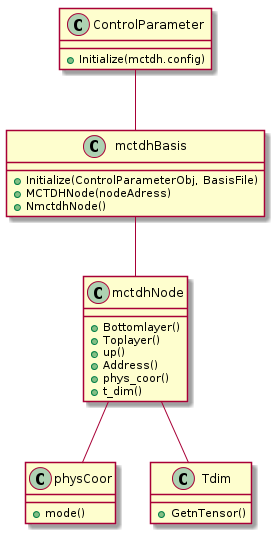
\includegraphics[scale=0.6]{figures/sequenceDiagram}
    \caption{Klassendiagramm der Programmierschnittstelle (API). Die Rechtecke repr"asentieren jeweils eine Klasse.
    Im oberen Bereich des Rechtecks befindet sich der Name der Klasse und im unteren Bereich eine Liste aller
    Memberfunktionen. F"ur eine detaillierte Beschreibung siehe Text.}\label{fig:uml_Cython}
\end{figure}



\section{Graphische Benutzeroberfl"ache f"ur MCTDH}

Zur Demonstration der graphischen Benutzeroberfl"ache wird im folgenden das Vorgehen zum Starten einer 
MCTDH Simulation vorgef"uhrt. Als Beispiel dient die Realzeitpro\-pagation eines Wellenpakets auf dem
ersten elektronisch angeregten Zustand ($S_1$) von NOCl.

\begin{figure}
    \centering
    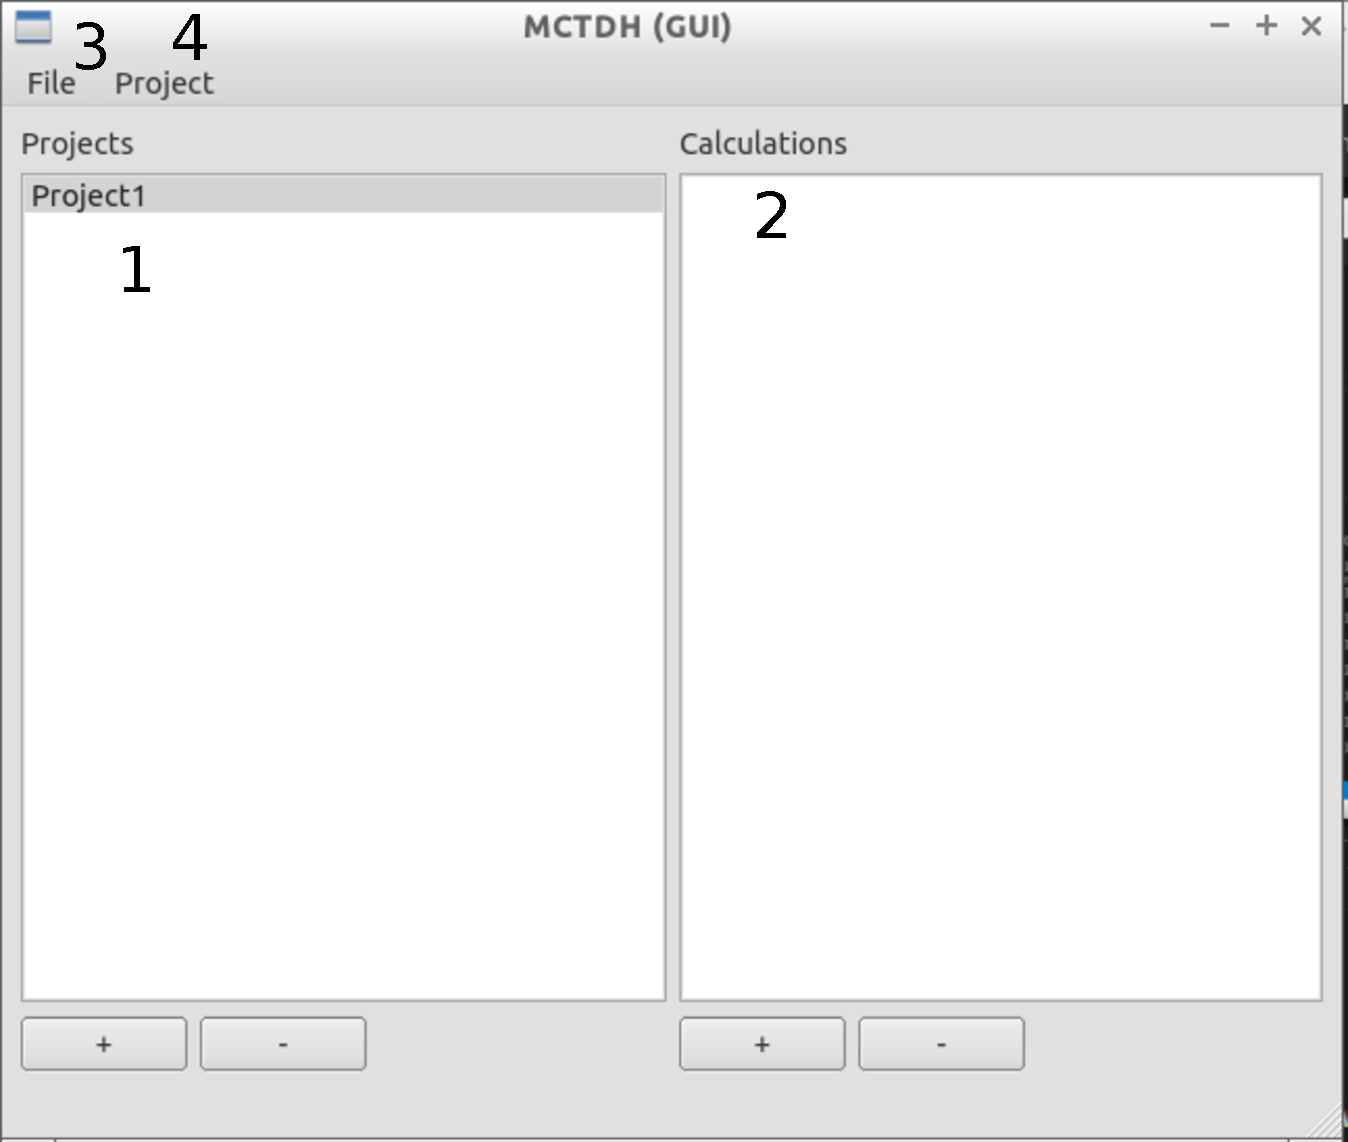
\includegraphics[scale=0.5]{figures/screenMain}
    \caption{Hauptfenster der MCTDH-GUI. Es zeigt aktuell vorhandene Projekte (\textbf{1}), sowie zugeh"orige Rechnungen (\textbf{2}).}\label{fig:workflow1}
\end{figure}

Beim Start der GUI erscheint das Hauptfenster (siehe Abbildung \ref{fig:workflow1}).
In Liste \textbf{1} sind alle vorhandenen Projekte aufgef"uhrt.
Nach Auswahl eines Projekts erscheinen in Liste \textbf{2} alle dem Projekt zugeoredneten Rechnungen.
Durch die Schaltfl"achen ,,+'' und ,,-'' k"onnen Projekte sowie Rechnungen jeweils hinzugef"ugt bzw.
entfernt werde.
Im Reiter ,,File'' (\textbf{3}) befinden sich zus"atzliche Optionen zur Projektverwaltung (siehe Abbildung \ref{fig:workflow2}).
Durch Klicken der Schaltfl"ache \textbf{5} wird ein neues Projekt erstellt. Externe Projekte werden durch die 
Schaltfl"ache \textbf{6} geladen. Bet"atigung der Schaltfl"ache \textbf{7} beendet die Benutzeroberfl"ache.

\begin{figure}
    \centering
    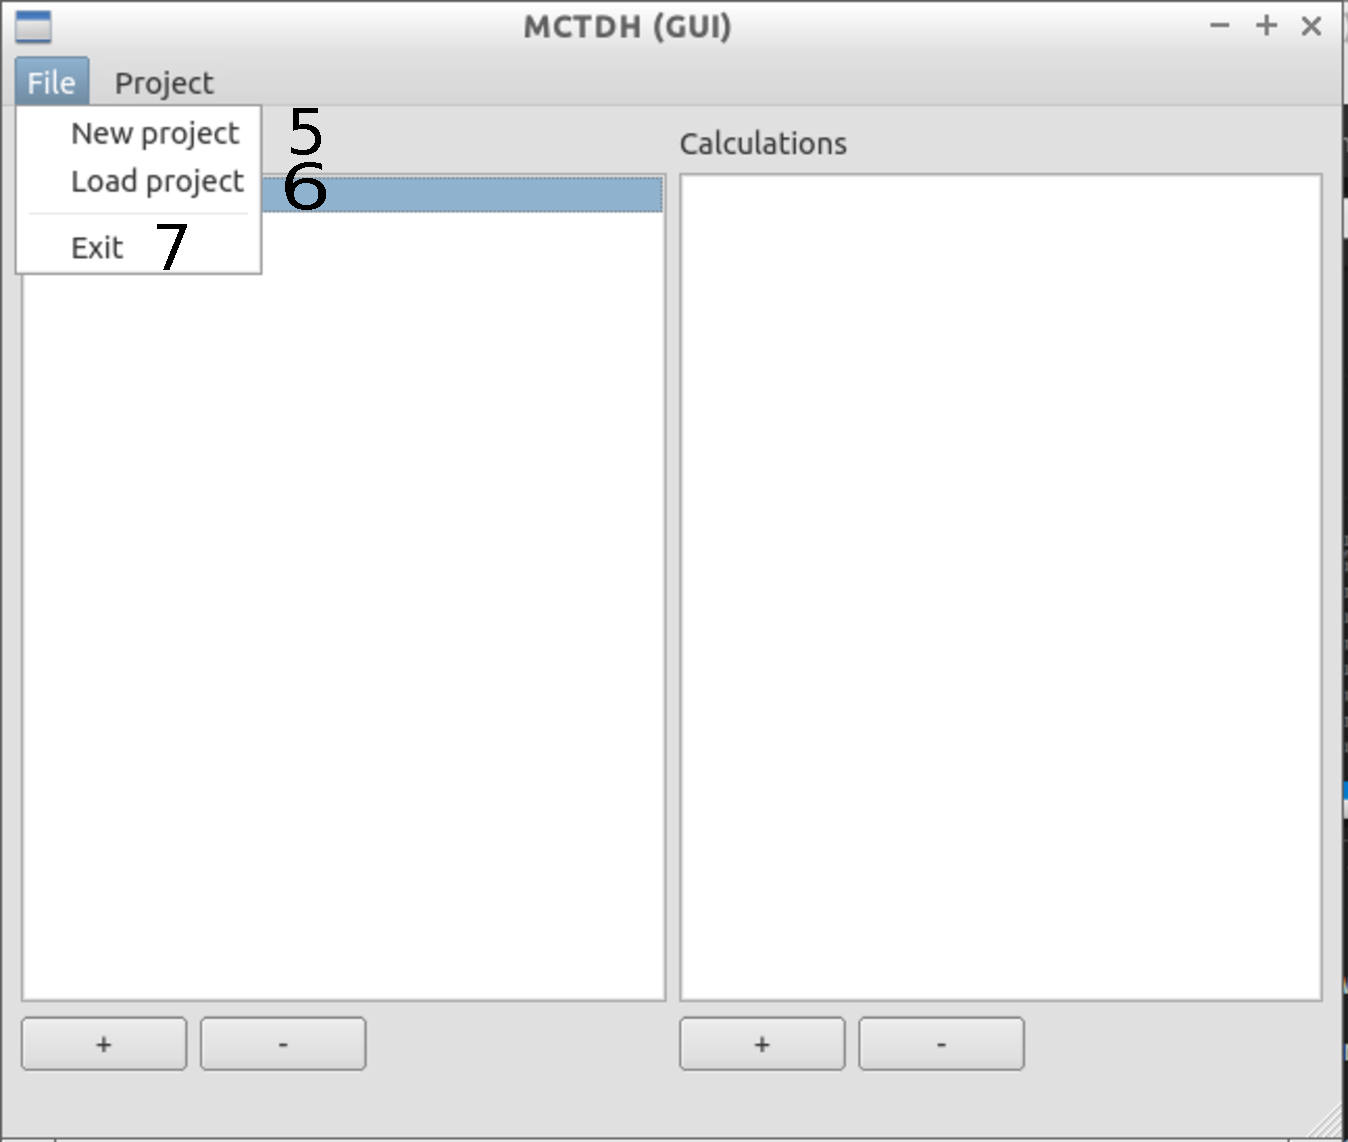
\includegraphics[scale=0.5]{figures/screenMainFile}
    \caption{Hauptfenster der MCTDH-GUI. Nach Bet"atigung des Reiters ,,File''
		stehen Optionen zur Projektverwaltung, sowie zum Beenden der GUI zur Verf"ugung.}\label{fig:workflow2}
\end{figure}

Zum Starten einer neuen Rechnung wird zuerst der Reiter ,,Project'' (Abbildung \ref{fig:workflow1} \textbf{4}) 
ausgew"ahlt. Zwei neue Buttons erscheinen (Abbildung \ref{fig:workflow3}). Durch Klicken von \textbf{8} 
erscheint ein neues Fenster mit dem Namen ,,MCTDH calculation'' (siehe Abbildung \ref{fig:workflow4}). 
In diesem Fenster wird die neue MCTDH Rechnung spezifiziert.

\begin{figure}
    \centering
    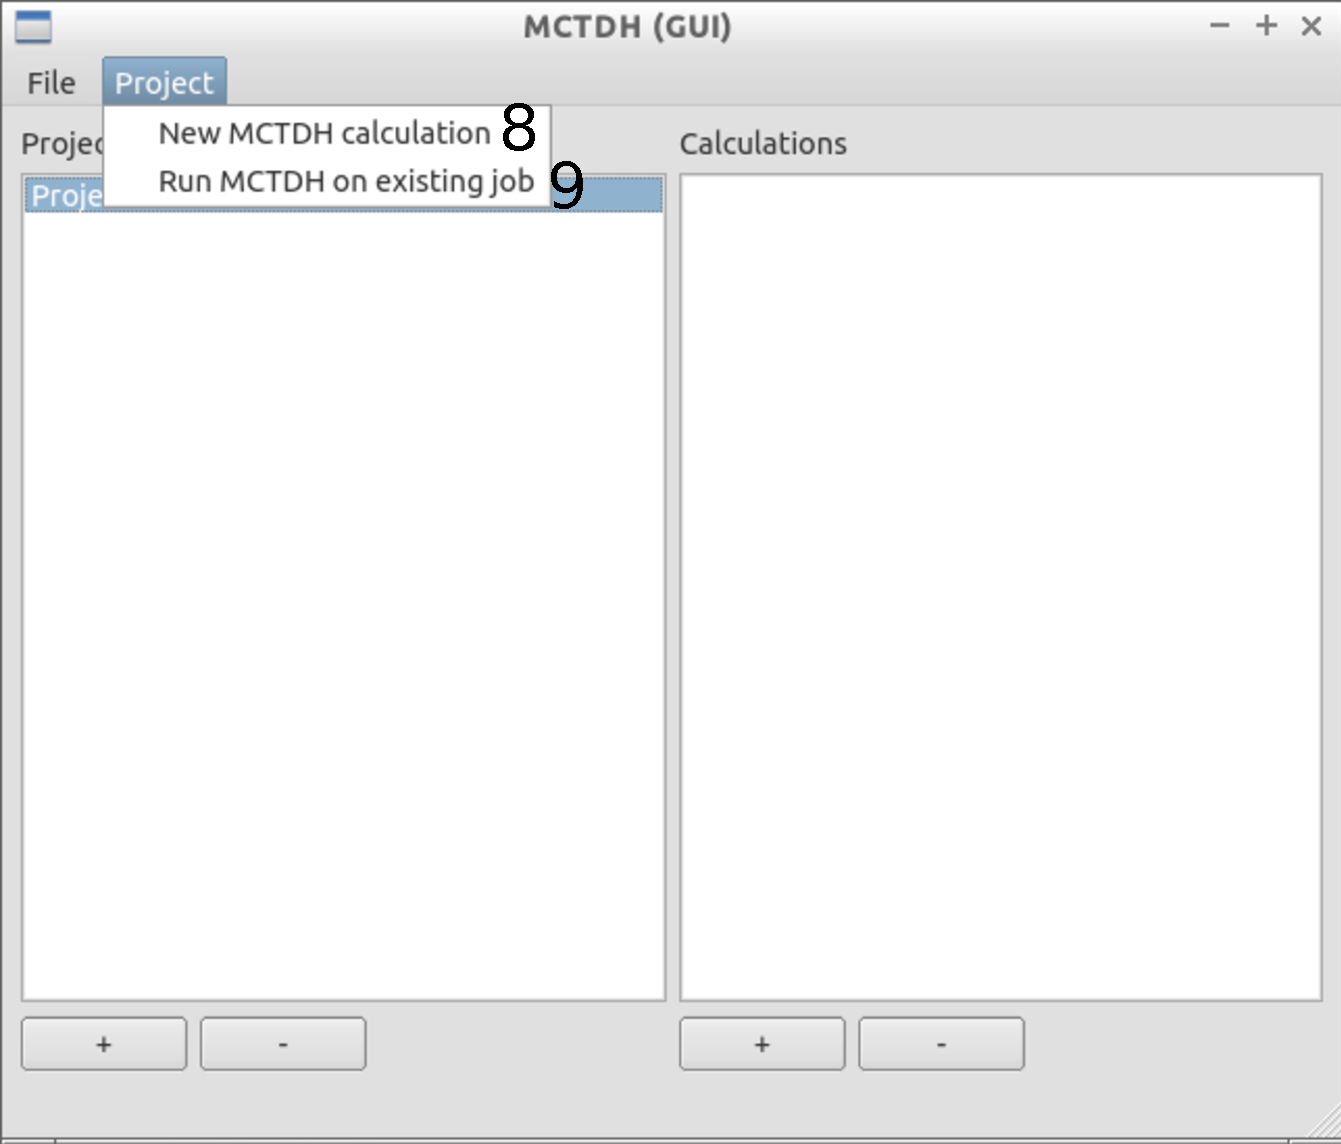
\includegraphics[scale=0.5]{figures/screenMainProject}
    \caption{Hauptfenster der MCTDH-GUI nach Bet"atigung des Reiters ,,Project''. Es stehen Optionen zum Erstellen und Starten einer
    MCTDH-Rechnung zur Verf"ugung.}\label{fig:workflow3}
\end{figure}

In dem Eingabefenster ,,MCTDH calculation'' kann im Feld \textbf{10} der Name der Rechnung angegeben werden. 
Sollte beim Speichern (Abbildung \ref{fig:workflow4} \textbf{18}) des MCTDH-Baums und der Einstellungsparameter 
kein Name angegeben sein, wird der Benutzer 
aufgefordert einen Name f"ur die Rechnung zu w"ahlen. 
%Bevor die Rechnung gespeichert wird, 
%wird "uberpr"uft, ob der gew"ahlte Name dem Namen einer andere Rechnung entspricht und, ob diese 
%dann gegebenfalls "uberschrieben werden soll.
Beim Speichern der Rechnung wird "uberpr"uft, ob eine Rechnung mit dem ausgew"ahlten Namen existiert,
um ein unabsichtliches "Uberschreiben zu verhindern.
In Liste \textbf{11} wird der entsprech\-ende Summe-von-Produkten Operator f"ur das gegebene System ausgew"ahlt.
"Uber die Kn"opfe  ,,on'' und ,,off'' (\textbf{12}) wird gesteuert, ob eine Potentialfl"achenauswertung mittels 
CDVR erfolgt.
Ist der ,,off'' Knopf aktiviert, werden keine Potentiale in der Liste \textbf{13} angezeigt.
Bei der Standardeinstellung der GUI ist der Knopf ,,on'' aktiviert und es k"onnen Potentiale durch Klicken
auf die Elemente der Liste \textbf{13} ausgew"ahlt werden. Im vorliegenden Beispiel wird die Option ,,off''
ausgew"ahlt.
Die Erweiterung der Summe-von-Produkten Operatoren und Potentialfl"achen kann schematisch erfolgen.

Mithilfe der MCTDH GUI k"onnen vier verschiedene Operationen durchgef"uhrt werden (\textbf{14}):
,,real-time propagation'', ,,imaginary-time propagation'', ,,Eigenstate calculation'' und ,,Thermal flux eigenstate calculation''.
Hier wird die Option ,,real-time propagation'' ausgew"ahlt.
Des Weiteren werden unter \textbf{15} Steuerungsparameter f"ur den Integrator ausgew"ahlt. Dazu geh"oren die Anfangszeit, die Endzeit,
der initiale Zeitschritt und (f"ur die Operationen ,,Eigenstate calculation'' und ,,Thermal flux eigenstate calculation'')
die Anzahl an Iterationen. Alle Parameter werden automatisch geladen, indem ein System aus
Liste \textbf{11} ausgew"ahlt wird oder eine Eingabe-Datei durch 
die ,,Load'' Schaltfl"alche \textbf{19} eingelesen wird. 
Der MCTDH-Baum, welcher die aktuell gew"ahlte Basis repr"asentiert, wird unter \textbf{16} 
als Listendiagramm angezeigt. Hier
kann durch Doppelklick die Anzahl der SPFs, der primitiven Basis und der Moden ver"andert werden.
Zus"atzlich wird der MCTDH-Baum in Form eines Diagramms in \textbf{17} angezeigt. 
Die Schaltfl"ache ,,Cancel'' \textbf{21} beendet das Eingabefenster
und die Schaltfl"ache ,,Start calculation'' (\textbf{20}) beginnt die MCTDH Simulation.
Alternativ kann die MCTDH Simulation auch aus dem Hauptfenster gestartet werden,
indem Schaltfl"ache ,,Run MCTDH on existing job'' (\textbf{9}) bet"atigt wird (siehe Abbildung \ref{fig:workflow3}).
%Durch Klicken der Schaltfl"ache ,,Run MCTDH on existing job'' (\textbf{9}) kann ebenfalls eine MCTDH Simulation gestartet.

In Abbildung \ref{fig:workflow5} wurde das System NOCl mit sinnvollen Eingabeparametern geladen,
indem auf ,,NOCl'' aus Liste \textbf{11} geklickt wurde.

\begin{figure}
    \centering
    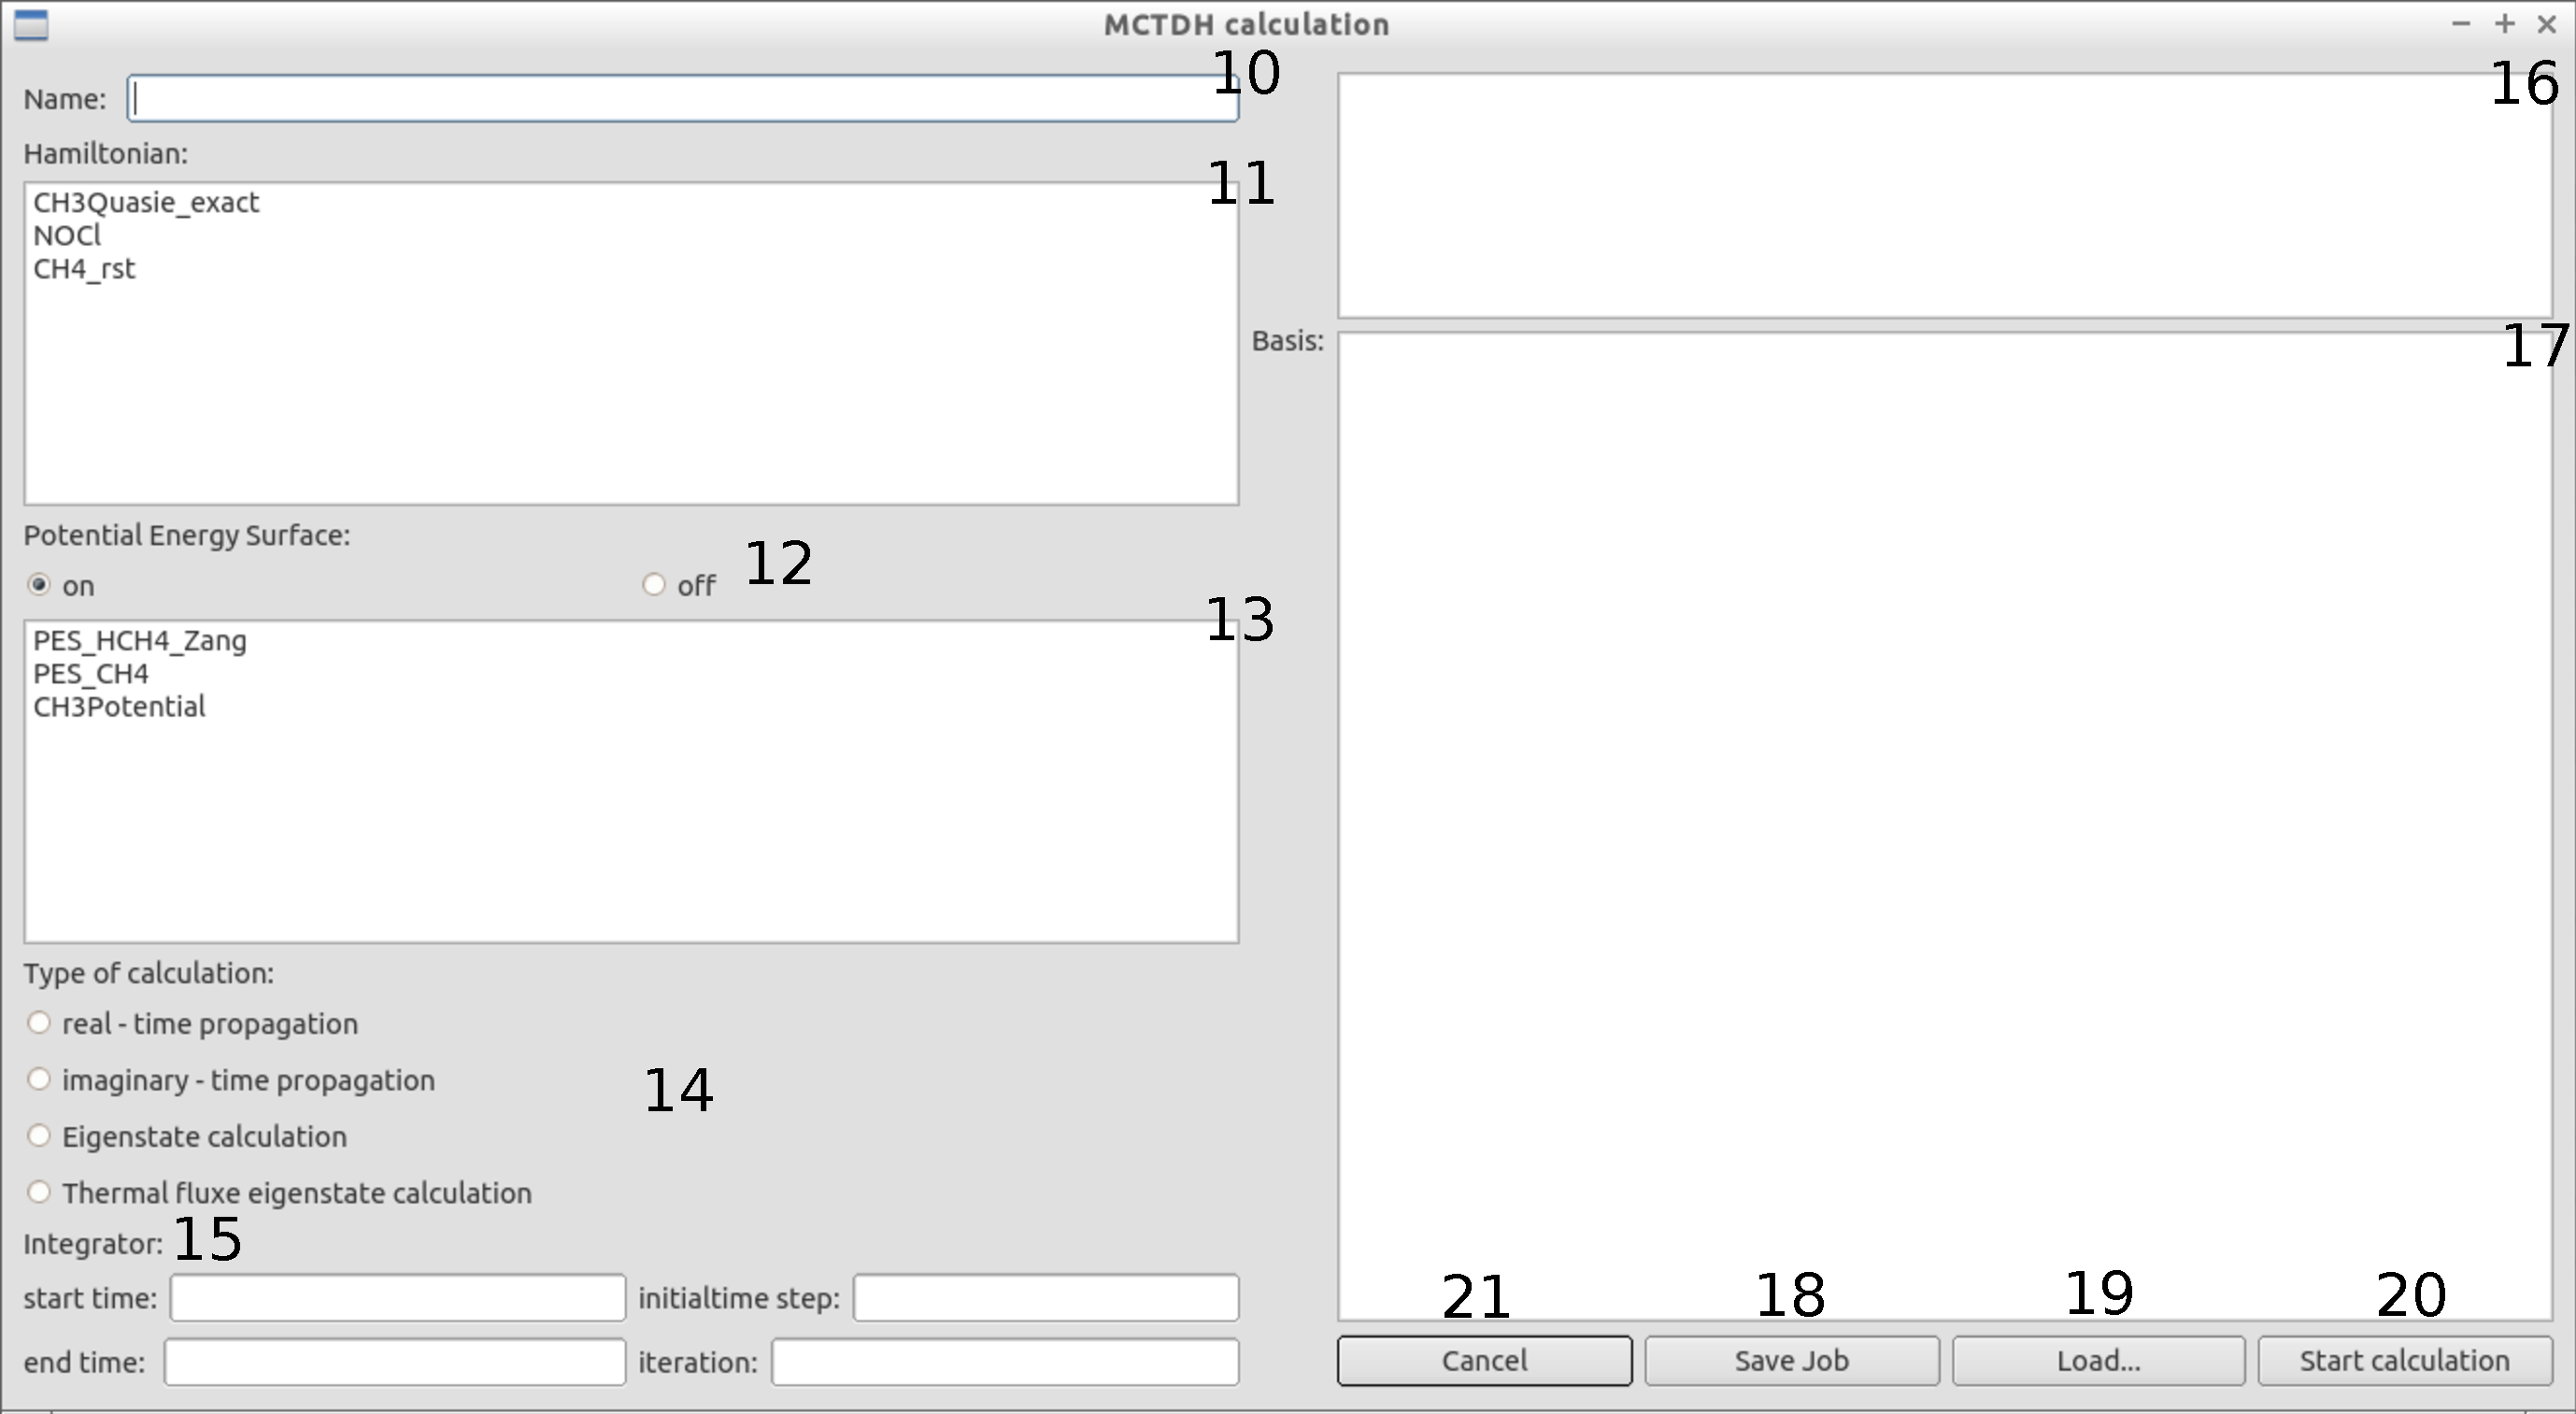
\includegraphics[angle=90, scale=0.45]{figures/screenWidgetA}
    \caption{Spezifikation einer neuen MCTDH-Rechnung durch die MCTDH-GUI.}\label{fig:workflow4}
\end{figure}
\begin{figure}
    \centering
    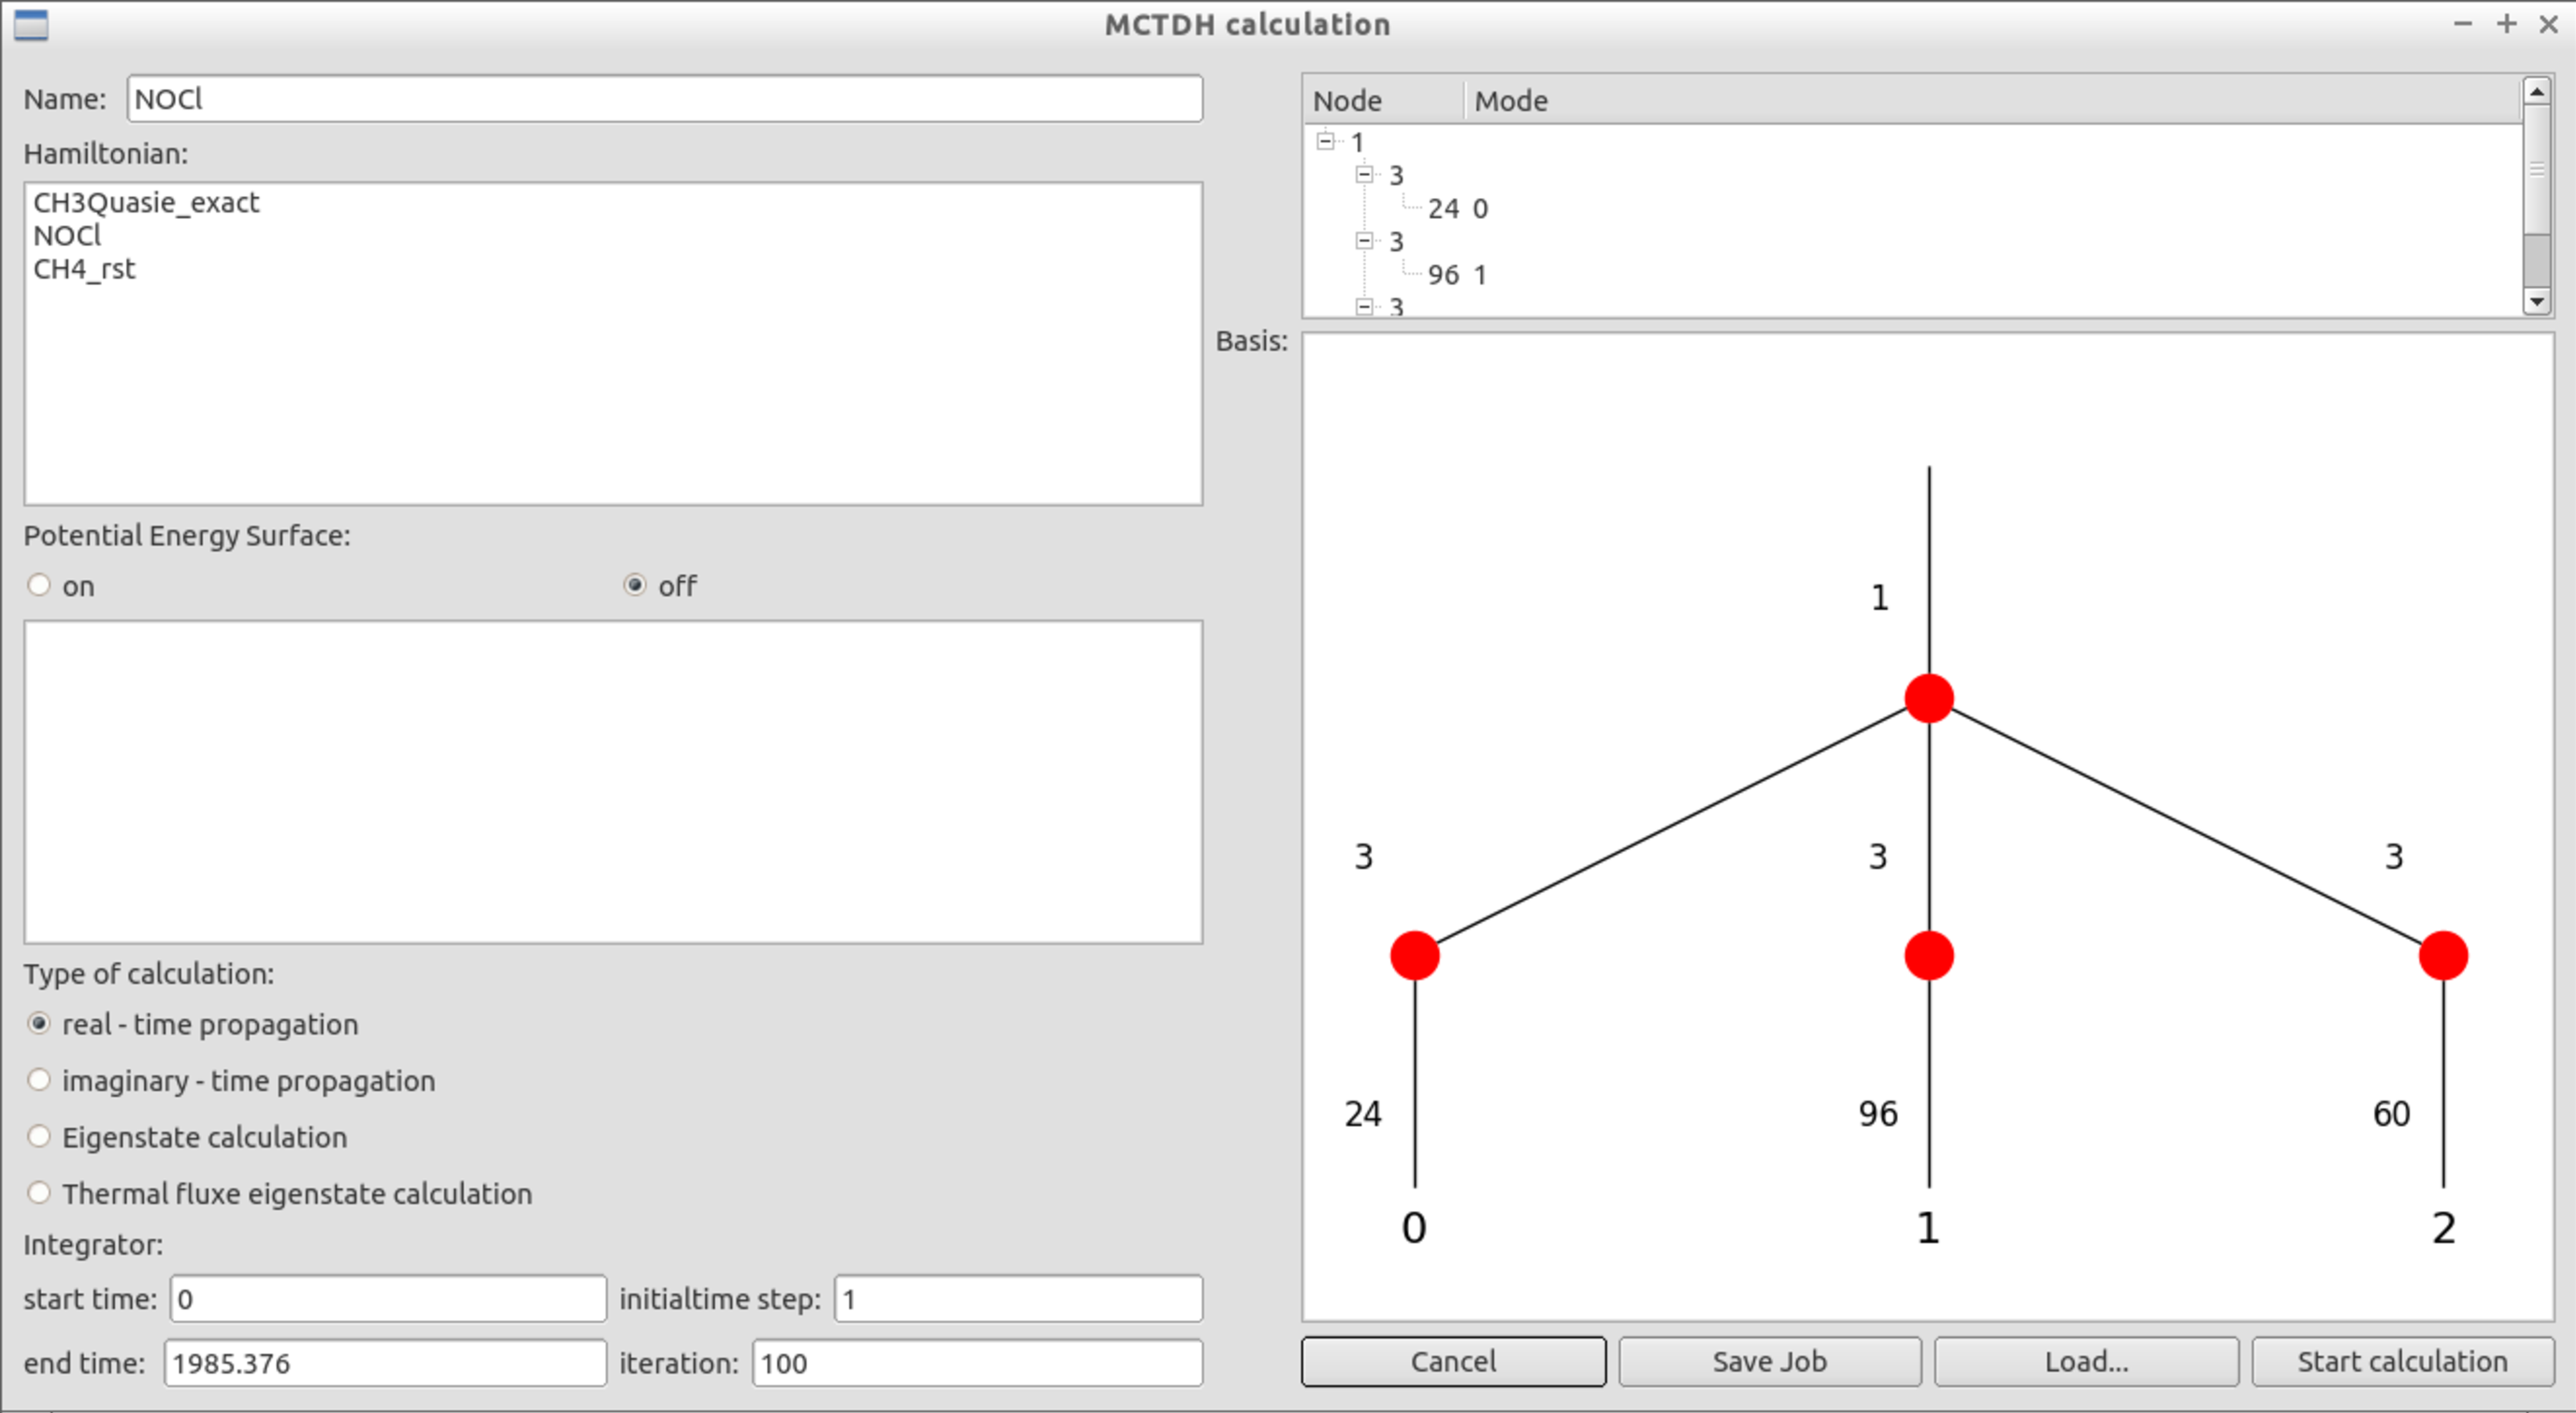
\includegraphics[angle=90, scale=0.45]{figures/screenWidgetAexample}
    \caption{Eingabefenster der MCTDH-GUI am Beispiel der
    Photodissoziation von NOCl.}\label{fig:workflow5}
\end{figure}
